\documentclass[a4paper]{article}

\usepackage[english]{babel}
\usepackage[utf8]{inputenc}
\usepackage{amsmath}
\usepackage{graphicx}
\usepackage[colorinlistoftodos]{todonotes}

\title{Gaussian processes applied to the study of chemotactic movements}

\author{Carlotta Porcelli, qbp693}

\date{\today}

\begin{document}
\maketitle

\begin{abstract}
Enter a short summary here. What topic do you want to investigate and why? What experiment did you perform? What were your main results and conclusion?
\end{abstract}

\section{Introduction 5 lines to max 1/2 page}
\label{sec:introduction}

Explain the context of the experiment here. Why is condensed matter physics interesting or important?
Optional things you could talk about (but don't have to -- this is up to you): transistors, computers, Quantum computers, fundamental knowledge (e.g. the resistance quantum).

Briefly explain what methods you will use in the experiment, and what values you will extract from the data.



\section{Theory 2-3 pages}
\label{sec:theory}

\subsection{The Gaussian Process}
Here, explain the concept of a 2-DEG in GaAs/AlGaAs. What is a 2-DEG and why does it arise?

\subsection{Hall Effect}
Explain the classical Hall effect in your own words. What do I measure at $B=0$? And what happens if $B>0$? Which effect gives rise to the voltage drop in the vertical direction?

\subsection{Quantum Hall Effect}
Explain the IQHE in your own words. What does the density of states look like in a 2-DEG when $B=0$? What are Landau levels and how do they arise? What are edge states? What does the electron transport look like when you change the magnetic field? What do you expect to measure?

\section{Matherials and Methods 1-2 pages}

\subsection{The data set}


\subsection{The library used}
When there is a danger of finding a local, rather than a global, maximum in the marginal likelihood, a non-zero value can be specified for n\_restarts\_optimizer, which will run the optimization algorithm as many times as specified, using randomly-chosen starting coordinates, in the hope that a globally-competitive value can be discovered.

\subsection{Choice of Kernel}
RBF - 
\subsubsection{Parameters}
\textbf{Lengthscale} \textit{l} describes how smooth a function is. Small lengthscale value means that function values can change quickly, large values characterize functions that change only slowly. Lengthscale also determines how far we can reliably extrapolate from the training data.
\\\textbf{Noise variance} \textit{${ \sigma  }_{ noise }^{ 2 }$} is formally not a part of the covariance function itself. It is used by the Gaussian process model to allow for noise present in training data. This parameter specifies how much noise is expected to be present in the data.



\section{Results and interpretation 2-3 pages}
Show a graph of the longitudinal resistivity ($\rho_{xx}$) and Hall resistivity ($\rho_{xy}$) versus magnetic field, extracted from the raw data shown in figure \ref{fig:data}. You will have the link to the data in your absalon messages, if not e-mail Guen (guen@nbi.dk). Explain how you calculated these values, and refer to the theory.

\begin{figure}
\centering
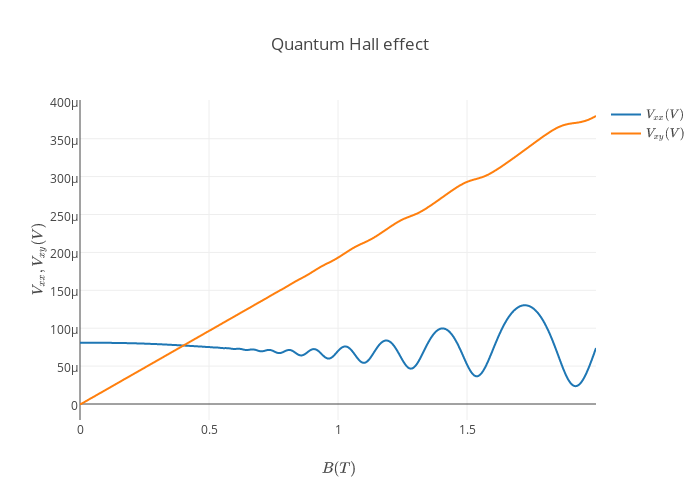
\includegraphics[width=1\textwidth]{raw_data.png}
\caption{\label{fig:data}Raw (unprocessed) data. Replace this figure with the one you've made, that shows the resistivity.}
\end{figure}


\section{Discussion 1/2-1 page}
Discuss your results. Compare the two values of $n_{s}$ that you've found in the previous section. Compare your results with literature and comment on the difference. If you didn't know the value of the resistance quantum, would you be able to deduce it from your measurements? If yes/no, why?

\subsection{Future work}

\newpage
\section{Some LaTeX tips}
\label{sec:latex}
\subsection{How to Include Figures}

First you have to upload the image file (JPEG, PNG or PDF) from your computer to writeLaTeX using the upload link the project menu. Then use the includegraphics command to include it in your document. Use the figure environment and the caption command to add a number and a caption to your figure. See the code for Figure \ref{fig:frog} in this section for an example.

\begin{figure}
\centering
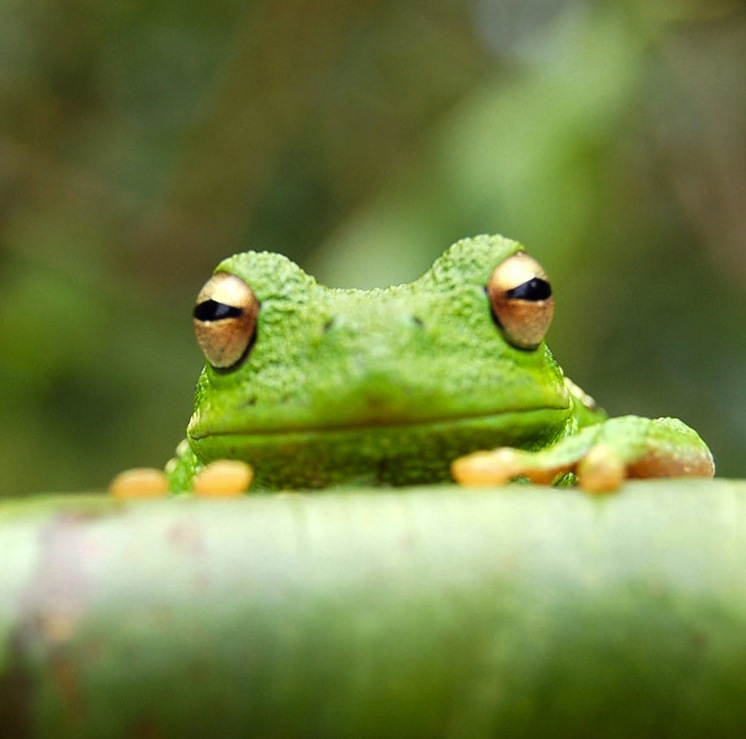
\includegraphics[width=0.3\textwidth]{frog.jpg}
\caption{\label{fig:frog}This frog was uploaded to writeLaTeX via the project menu.}
\end{figure}

\subsection{How to Make Tables}

Use the table and tabular commands for basic tables --- see Table~\ref{tab:widgets}, for example.

\begin{table}
\centering
\begin{tabular}{l|r}
Item & Quantity \\\hline
Widgets & 42 \\
Gadgets & 13
\end{tabular}
\caption{\label{tab:widgets}An example table.}
\end{table}

\subsection{How to Write Mathematics}

\LaTeX{} is great at typesetting mathematics. Let $X_1, X_2, \ldots, X_n$ be a sequence of independent and identically distributed random variables with $\text{E}[X_i] = \mu$ and $\text{Var}[X_i] = \sigma^2 < \infty$, and let

\begin{equation}
S_n = \frac{X_1 + X_2 + \cdots + X_n}{n}
      = \frac{1}{n}\sum_{i}^{n} X_i
\label{eq:sn}
\end{equation}

denote their mean. Then as $n$ approaches infinity, the random variables $\sqrt{n}(S_n - \mu)$ converge in distribution to a normal $\mathcal{N}(0, \sigma^2)$.

The equation \ref{eq:sn} is very nice.

\subsection{How to Make Sections and Subsections}

Use section and subsection commands to organize your document. \LaTeX{} handles all the formatting and numbering automatically. Use ref and label commands for cross-references.

\subsection{How to Make Lists}

You can make lists with automatic numbering \dots

\begin{enumerate}
\item Like this,
\item and like this.
\end{enumerate}
\dots or bullet points \dots
\begin{itemize}
\item Like this,
\item and like this.
\end{itemize}
\dots or with words and descriptions \dots
\begin{description}
\item[Word] Definition
\item[Concept] Explanation
\item[Idea] Text
\end{description}

We hope you find write\LaTeX\ useful, and please let us know if you have any feedback using the help menu above.

\begin{thebibliography}{9}
\bibitem{nano3}
  K. Grove-Rasmussen og Jesper Nygård,
  \emph{Kvantefænomener i Nanosystemer}.
  Niels Bohr Institute \& Nano-Science Center, Københavns Universitet

\end{thebibliography}
\end{document}